\documentclass[]{jarticle}          % 一段組
%\documentclass[twocolumn]{jarticle} % 二段組

\textwidth 180mm
\textheight 255mm
\oddsidemargin -12mm
\topmargin -15mm
\columnsep 10mm

%\vspace{0.5cm} % 一段組の場合はコメントアウトした方が体裁がよいx
%] % 一段組の場合はコメントアウトする

\usepackage{styles/labheadings}
\usepackage[dvipdfmx]{graphicx,color}
\usepackage{amsmath,amssymb}
\usepackage{url}
% 追加
\usepackage{listings,jvlisting} 
\usepackage[hang,small,bf]{caption}
\usepackage[subrefformat=parens]{subcaption}
\captionsetup{compatibility=false}

\newcommand{\aU}{\mbox{\boldmath $a$}}
\newcommand{\bU}{\mbox{\boldmath $b$}}
\newcommand{\cU}{\mbox{\boldmath $c$}}
\newcommand{\dU}{\mbox{\boldmath $d$}}
\newcommand{\eU}{\mbox{\boldmath $e$}}
\newcommand{\fU}{\mbox{\boldmath $f$}}
\newcommand{\gU}{\mbox{\boldmath $g$}}
\newcommand{\hU}{\mbox{\boldmath $h$}}
\newcommand{\iU}{\mbox{\boldmath $i$}}
\newcommand{\jU}{\mbox{\boldmath $j$}}
\newcommand{\kU}{\mbox{\boldmath $k$}}
\newcommand{\lU}{\mbox{\boldmath $l$}}
\newcommand{\mU}{\mbox{\boldmath $m$}}
\newcommand{\nU}{\mbox{\boldmath $n$}}
\newcommand{\oU}{\mbox{\boldmath $o$}}
\newcommand{\pU}{\mbox{\boldmath $p$}}
\newcommand{\qU}{\mbox{\boldmath $q$}}
\newcommand{\rU}{\mbox{\boldmath $r$}}
\newcommand{\sU}{\mbox{\boldmath $s$}}
\newcommand{\tU}{\mbox{\boldmath $t$}}
\newcommand{\uU}{\mbox{\boldmath $u$}}
\newcommand{\vU}{\mbox{\boldmath $v$}}
\newcommand{\wU}{\mbox{\boldmath $w$}}
\newcommand{\xU}{\mbox{\boldmath $x$}}
\newcommand{\yU}{\mbox{\boldmath $y$}}
\newcommand{\zU}{\mbox{\boldmath $z$}}
\newcommand{\AU}{\mbox{\boldmath $A$}}
\newcommand{\BU}{\mbox{\boldmath $B$}}
\newcommand{\CU}{\mbox{\boldmath $C$}}
\newcommand{\DU}{\mbox{\boldmath $D$}}
\newcommand{\EU}{\mbox{\boldmath $E$}}
\newcommand{\FU}{\mbox{\boldmath $F$}}
\newcommand{\GU}{\mbox{\boldmath $G$}}
\newcommand{\HU}{\mbox{\boldmath $H$}}
\newcommand{\IU}{\mbox{\boldmath $I$}}
\newcommand{\JU}{\mbox{\boldmath $J$}}
\newcommand{\KU}{\mbox{\boldmath $K$}}
\newcommand{\LU}{\mbox{\boldmath $L$}}
\newcommand{\MU}{\mbox{\boldmath $M$}}
\newcommand{\NU}{\mbox{\boldmath $N$}}
\newcommand{\OU}{\mbox{\boldmath $O$}}
\newcommand{\PU}{\mbox{\boldmath $P$}}
\newcommand{\QU}{\mbox{\boldmath $Q$}}
\newcommand{\RU}{\mbox{\boldmath $R$}}
\newcommand{\SU}{\mbox{\boldmath $S$}}
\newcommand{\TU}{\mbox{\boldmath $T$}}
\newcommand{\UU}{\mbox{\boldmath $U$}}
\newcommand{\VU}{\mbox{\boldmath $V$}}
\newcommand{\WU}{\mbox{\boldmath $W$}}
\newcommand{\XU}{\mbox{\boldmath $X$}}
\newcommand{\YU}{\mbox{\boldmath $Y$}}
\newcommand{\ZU}{\mbox{\boldmath $Z$}}
\newcommand{\epU}{\mbox{\boldmath $\epsilon$}}
\newcommand{\taU}{\mbox{\boldmath $\tau$}}
\newcommand{\etU}{\mbox{\boldmath $\eta$}}
\newcommand{\xiU}{\mbox{\boldmath $\xi$}}
\newcommand{\wwU}{\mbox{\boldmath $\omega$}}
\newcommand{\WwU}{\mbox{\boldmath $\Omega$}}
\newcommand{\lmU}{\mbox{\boldmath $\lambda$}}
\newcommand{\LmU}{\mbox{\boldmath $\Lambda$}}
\newcommand{\PiU}{\mbox{\boldmath $\Pi$}}
\newcommand{\SgU}{\mbox{\boldmath $\Sigma$}}
\newcommand{\thU}{\mbox{\boldmath $\theta$}}
\newcommand{\ThU}{\mbox{\boldmath $\Theta$}}
\newcommand{\roU}{\mbox{\boldmath $\rho$}}
\newcommand{\nuU}{\mbox{\boldmath $\nu$}}
\newcommand{\ones}{{\bf 1}}
\newcommand{\zr}{{\bf 0}}
\newcommand{\eq}{\begin{equation}}
\newcommand{\en}{\end{equation}}
\newcommand{\eqa}{\begin{eqnarray}}
\newcommand{\ena}{\end{eqnarray}}
\newcommand{\xx}{\makebox[1cm]{}}
\newcommand{\xm}{\makebox[0.5cm]{}}
\newcommand{\x}{\makebox[0.2cm]{}}
\newcommand{\tr}{{\rm tr}}
\newcommand{\sgn}{{\rm sgn}}
\newcommand{\ad}{{\rm ad}}

\newcommand{\rank}{{\rm rank}}
\newcommand{\diag}{{\rm diag}}
\newcommand{\lbr}{\left(\begin{array}}
\newcommand{\rbr}{\end{array}\right)}
\newcommand{\Proof}{\noindent{\em Proof\/}}
\newcommand{\Solution}{\noindent{\em Solution}}
\newcommand{\Derivation}{\noindent{\em Derivation}}
\newcommand{\msp}{\vspace*{\medskipamount}\\}
\newcommand{\qed}{\hspace*{\fill}$\Box$}
\newcommand{\aX}{{\bf a}}
\newcommand{\bX}{{\bf b}}
\newcommand{\cX}{{\bf c}}
\newcommand{\dX}{{\bf d}}
\newcommand{\eX}{{\bf e}}
\newcommand{\fX}{{\bf f}}
\newcommand{\gX}{{\bf g}}
\newcommand{\hX}{{\bf h}}
\newcommand{\iX}{{\bf i}}
\newcommand{\jX}{{\bf j}}
\newcommand{\kX}{{\bf k}}
\newcommand{\lX}{{\bf l}}
\newcommand{\mX}{{\bf m}}
\newcommand{\nX}{{\bf n}}
\newcommand{\oX}{{\bf o}}
\newcommand{\pX}{{\bf p}}
\newcommand{\qX}{{\bf q}}
\newcommand{\rX}{{\bf r}}
\newcommand{\sX}{{\bf s}}
\newcommand{\tX}{{\bf t}}
\newcommand{\uX}{{\bf u}}
\newcommand{\vX}{{\bf v}}
\newcommand{\wX}{{\bf w}}
\newcommand{\xX}{{\bf x}}
\newcommand{\yX}{{\bf y}}
\newcommand{\zX}{{\bf z}}
\newcommand{\AX}{{\bf A}}
\newcommand{\BX}{{\bf B}}
\newcommand{\CX}{{\bf C}}
\newcommand{\DX}{{\bf D}}
\newcommand{\EX}{{\bf E}}
\newcommand{\FX}{{\bf F}}
\newcommand{\GX}{{\bf G}}
\newcommand{\HX}{{\bf H}}
\newcommand{\IX}{{\bf I}}
\newcommand{\JX}{{\bf J}}
\newcommand{\KX}{{\bf K}}
\newcommand{\LX}{{\bf L}}
\newcommand{\MX}{{\bf M}}
\newcommand{\NX}{{\bf N}}
\newcommand{\OX}{{\bf O}}
\newcommand{\PX}{{\bf P}}
\newcommand{\QX}{{\bf Q}}
\newcommand{\RX}{{\bf R}}
\newcommand{\SX}{{\bf S}}
\newcommand{\TX}{{\bf T}}
\newcommand{\UX}{{\bf U}}
\newcommand{\VX}{{\bf V}}
\newcommand{\WX}{{\bf W}}
\newcommand{\XX}{{\bf X}}
\newcommand{\YX}{{\bf Y}}
\newcommand{\ZX}{{\bf Z}}

% report.texと同じディレクトリにnumerical_definition.texを入れておけば上の書き方でもいいはずです

\usepackage[
  dvipdfm,
  bookmarks=true,
  bookmarksnumbered=true,
  colorlinks=true]{hyperref}
\AtBeginDvi{\special{pdf:tounicode EUC-UCS2}}

%ここからソースコードの表示に関する設定
\lstset{
  basicstyle={\ttfamily},
  identifierstyle={\small},
  commentstyle={\smallitshape},
  keywordstyle={\small\bfseries},
  ndkeywordstyle={\small},
  stringstyle={\small\ttfamily},
  frame={tb},
  breaklines=true,
  columns=[l]{fullflexible},
  numbers=left,
  xrightmargin=0zw,
  xleftmargin=3zw,
  numberstyle={\scriptsize},
  stepnumber=1,
  numbersep=1zw,
  lineskip=-0.5ex
}
%ここまでソースコードの表示に関する設定

\pagestyle{labheadings}
\headerleft{進捗報告}   % ヘッダの左側のタイトル
\headerright{2023年05月28日}  % ヘッダの右側のタイトル

\begin{document}

%\twocolumn % 一段組の場合はコメントアウトする

\vspace*{2ex}
\begin{center}
 {\Large \bf 進捗報告}\\ % タイトル
 \vspace*{5mm}
 {\large B4 田川幸汰}% 発表者名
\end{center}

%\vspace{0.5cm} % 一段組の場合はコメントアウトした方が体裁がよいx
%] % 一段組の場合はコメントアウトする

%新しく作成したコマンド
% \newcommand{\reffig}[1]{\hyperref[#1]{図\ref{#1}}}
% \newcommand{\refeq}[1]{\hyperref[#1]{式(\ref{#1})}}
% \newcommand{\reftab}[1]{\hyperref[#1]{表\ref{#1}}}
% \newcommand{\refsec}[1]{\hyperref[#1]{\ref{#1}章}}
% \newcommand{\refsubsec}[1]{\hyperref[#1]{\ref{#1}節}}

\section{概要}
 課題2と課題3についての進捗報告を行う。\\
 課題2では、全方位画像を撮影して, その画像から指定した方向の透視投影画像を生成する。
この課題を通して正距円筒画像から透視絵投影画像の生成方法について学習する。 \\
 課題3ではbashのスクリプトと課題2で作成したプログラムを用いて,水平方向の視線を$-\pi$から$\pi$まで
10度刻みで変化させた透視投影画像を生成する。
この課題を通してシェルスクリプトの使い方について学習する。 \\

\section{課題2.全方位画像から透視投影画像生成}
実装方法と理論について、以下の節でまとめる。

\subsection{課題2の実装方法}
以下に全方位画像から透視投影画像を生成する方法をまとめる\cite{bib_1}。詳しい理論については以降の節で説明する。
\begin{itemize}
  \item 入力...正距円筒画像${I_e}$、水平方向及び垂直方向の画角${\Theta,\Phi}$、視線角度 ${\theta_{eye},\phi_{eye},\psi_{eye}}$
  \item 出力...透視投影画像${I_p}$
  \item アルゴリズム
  \begin{enumerate}
    \item 出力画像サイズ $W_{p}$ , $H_{p}$ を計算する。
    \item 水平方向、垂直方向の画素間の長さ${Δx,Δy}$を計算する。
    \item 透視投影画像${I_p}$の画素${(u_p,v_p)}$から、3次元の視線ベクトル$\xU$を計算する。
    \item 視線ベクトル $\xU$ を回転行列 $R(\theta_{eye},\phi_{eye})$ 、$R(\psi_{eye})$ により回転する。
    \item 4.で求めた視線ベクトル$\xU$から、${(\theta,\phi)}$を計算する。
    \item 正距円筒画像${I_e}$上の対応する画素${(u_e,v_e)}$を計算して、その画素値を透視投影画像${I_p}$の画素${(u_p,v_p)}$に割り当てる。
  \end{enumerate}
\end{itemize}

\subsection{画素間の長さ}
水平、垂直方向の画角${\Theta,\Phi}$と画像サイズ${W_p,H_p}$が与えられているとき、
画像面までの距離を1(${z=1})$とすると、水平方向、垂直方向の画素間の長さ${Δx,Δy}$は次のように与えられる。

\begin{equation}
  Δx = 2\tan(\Theta/2)/W_p
  \label{eq7}
\end{equation}

\begin{equation}
  Δy = 2\tan(\Phi/2)/H_p
  \label{eq8}
\end{equation}

\subsection{視線ベクトルの計算}
透視投影画像の画素${(u_p,v_p)}$とすると、\hyperref[eq7]{式(\ref{eq7})}、\hyperref[eq8]{式(\ref{eq8})}
で求めた${Δx,Δy}$を用いて3次元の視線ベクトル${\xU}$は次のように与えられる。
\begin{equation}
  \xU = 
  \left( \begin{array}{cc}
  x \\ y \\ z
  \end{array} \right) =
  \left( \begin{array}{cc}
  (u_p-W_p/2)Δx \\ (v_p-H_p/2)Δy \\ 1
  \end{array} \right) 
  \label{eq9}
\end{equation}

\subsection{透視投影画像への投影}
正距円筒画像の一部を透視画像の画像面に投影することを考える。
正距円筒画像は球面上に投影した画像とも考えられるので、
透視投影の画像面の画素に対応する正距円筒画像の角度情報が得られれば、
正距円筒画像の画素を透視投影画像に投影できる。\\
透視投影面上の座標と角度${(\theta,\phi,\psi)}$の関係を下の\hyperref[graphone]{図\ref{graphone}}に示す。\\
\begin{figure}[!ht]
  \begin{center}
    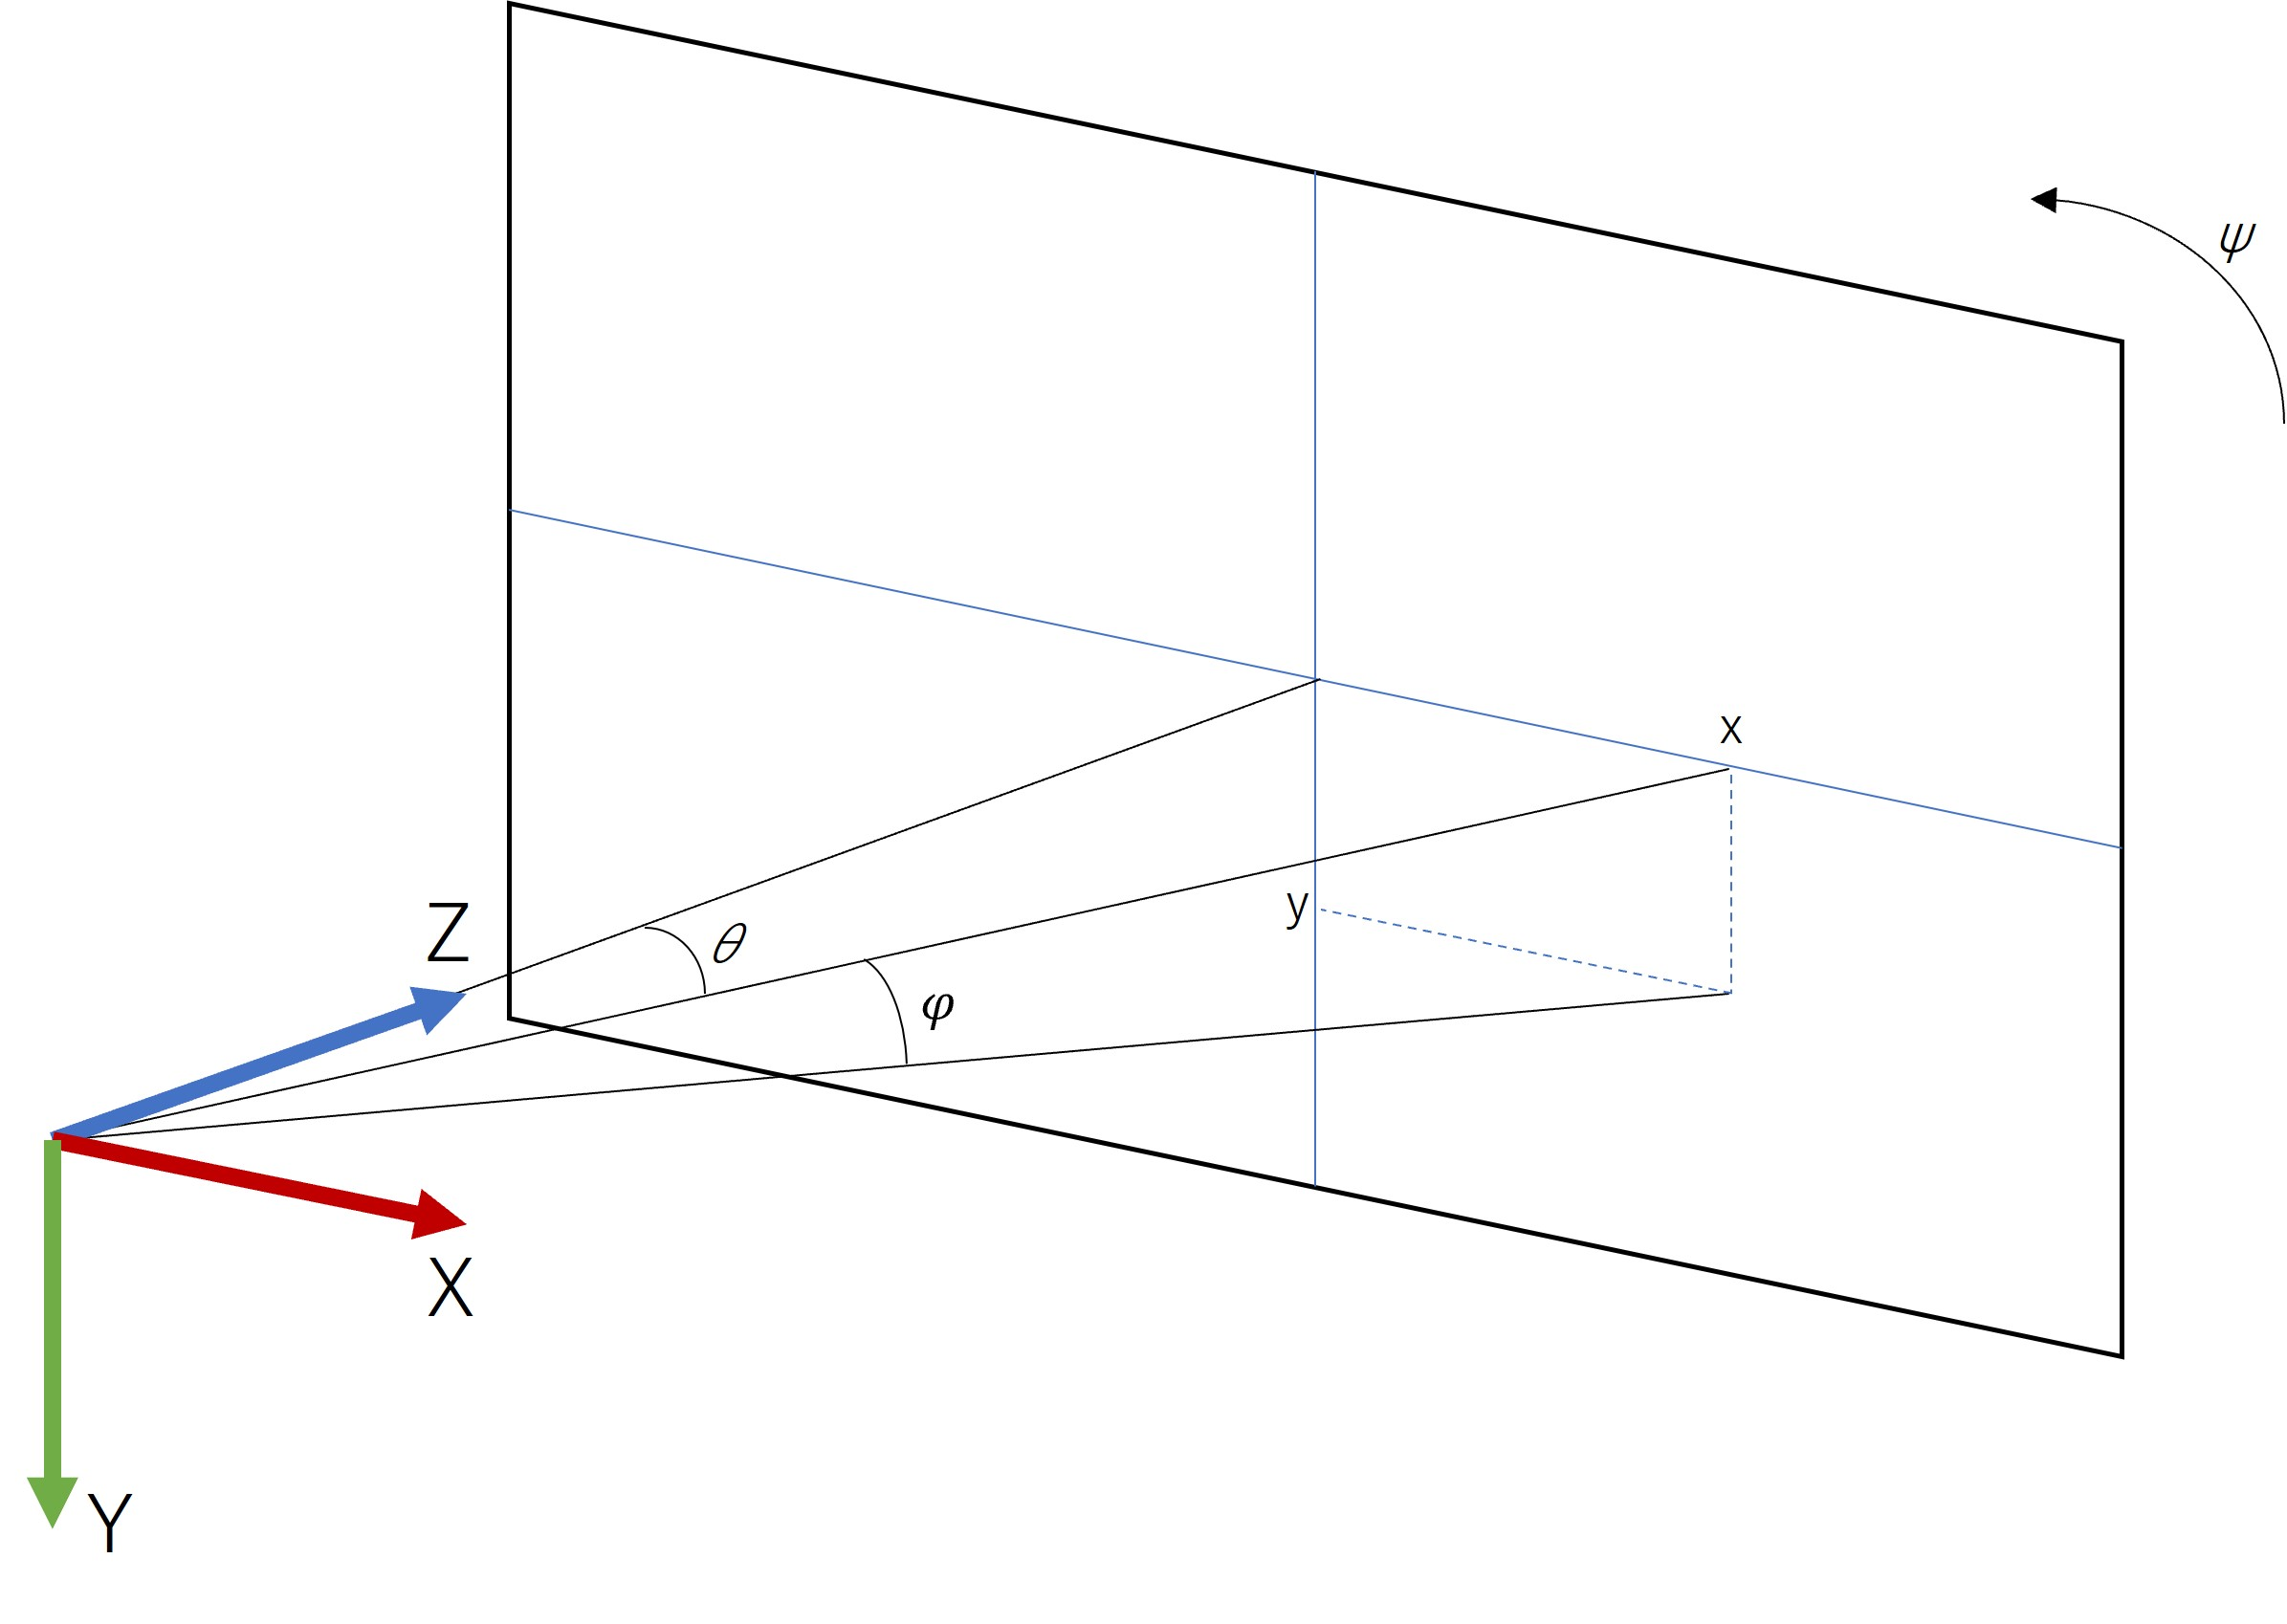
\includegraphics[scale=0.8]{figures/kadai2_graph.jpg}
    \caption{角度の定義}
    \label{graphone}
  \end{center}
\end{figure}
上記の定義より、\hyperref[eq9]{式(\ref{eq9})}で求めた透視投影面上の座標${(x,y,z)}$から、
角度${(\theta,\phi)}$は次のように与えられる。

\begin{equation}
  \theta = \tan^{-1}\frac{x}{z}
  \label{eq10}
\end{equation}

\begin{equation}
  \phi = -\tan^{-1}\frac{y}{\sqrt{x^{2}+z^{2}}}
  \label{eq11}
\end{equation}

ただし、${X}$軸周りの回転は${Y}$軸から${Z}$軸方向への回転が正の回転であることを考えて、
${\phi}$の符号は反転している。

\subsection{360度画像の座標系変換}
360度カメラで撮影した画像は、正距円筒画像として保存される。
これはシーンを球面に投影したものを緯度、軽度を画像の縦方向と横方向に対応付けて矩形の画像として再現したものである。\\
カメラ画像の${Z}$軸(光軸)が正距円筒画像の中心を通るとき、画像中心の$\theta$-$\phi$座標系での座標が${(\theta,\phi)=(0,0)}$となると考えると、
画像の左上を原点として、右方向に${u}$軸、下方向に${v}$軸をとる座標系との関係は次のように表せる。

\begin{equation}
  (\theta,\phi)=((u-\frac{W}{2})\frac{2\pi}{W},(\frac{H}{2}-v)\frac{\pi}{H})
  \label{eq12}
\end{equation}
\begin{equation}
  (u,v)=((\theta+\pi)\frac{W}{2\pi},(\frac{\pi}{2}-\phi)\frac{H}{\pi})
  \label{eq13}
\end{equation}

ここで、$W$及び$H$は入力画像の幅及び高さである。

\subsection{画像サイズの決定}
入力画像の解像度に合わせて出力画像を生成する場合、画角に応じた適切な画像サイズを計算する必要がある。
入力画像の横サイズ $W_{e}$ 及び縦サイズ $H_{e}$ 、
出力画像の水平、垂直方向の画角 $(\Theta,\Phi)$ が与えられているとき、
画像の横サイズ$W_{p}$ 及び縦サイズ $H_{p}$ は次のように与えられる。

\begin{equation}
  W_{p}=2\tan(\frac{\Theta}{2})\frac{W_{e}}{2\pi}
  \label{eq14}
\end{equation}
\begin{equation}
  H_{p}=2\tan(\frac{\Phi}{2})\frac{H_{e}}{\pi}
  \label{eq15}
\end{equation}

\subsection{視点移動}
画像面の回転がない場合、視点方向 $\vU=(0,0,1)^{\top}$である。
視点の回転を行う場合、まず $X$ 軸周りに $\phi_{eye}$ だけ回転したあと、
$Y$ 軸周りに $\theta_{eye}$ だけ回転すれば良い。
したがって、そのための回転行列は次のように与えられる。

\begin{equation}
  R(\theta_{eye},\phi_{eye})=
  \begin{pmatrix}
    \cos\theta_{eye} & 0 & \sin\theta_{eye} \\
    0 & 1 & 0 \\
    -\sin\theta_{eye} & 0 &
    \cos\theta_{eye}
  \end{pmatrix}
  \begin{pmatrix}
    1 & 0 & 0 \\
    0 & \cos\phi_{eye} & 
    -\sin\phi_{eye} \\
    0 & \sin\phi_{eye} &
    \cos\phi_{eye}
  \end{pmatrix}
  \label{eq16}
\end{equation}

また、光軸周りに $\psi_{eye}$ だけ画像面を回転する場合、
視点方向 $\vU$ を $R(\theta_{eye},\phi_{eye})$ で回転したあとのベクトルを
新たに回転軸として回転を行えばよい。新たな回転軸 $\lU$ 周りの回転行列は、
ロドリゲスの定理より次のように与えられる。

\begin{equation}
  \scriptsize
  R(\psi_{eye})=
  \begin{pmatrix}
    l_{x}^{2}(1-\cos\psi_{eye})+\cos\psi_{eye} &
    l_{x}l_{y}(1-\cos\psi_{eye})-l_{z}\sin\psi_{eye} &
    l_{z}l_{x}(1-\cos\psi_{eye})+l_{y}\sin\psi_{eye} \\
    l_{x}l_{y}(1-\cos\psi_{eye})+l_{z}\sin\psi_{eye}&
    l_{y}^{2}(1-\cos\psi_{eye})+\cos\psi_{eye} &
    l_{y}l_{z}(1-\cos\psi_{eye})-l_{x}\sin\psi_{eye} \\
    l_{z}l_{x}(1-\cos\psi_{eye})-l_{y}\sin\psi_{eye} &
    l_{y}l_{z}(1-\cos\psi_{eye})+l_{x}\sin\psi_{eye} &
    l_{z}^{2}(1-\cos\psi_{eye})+\cos\psi_{eye}
  \end{pmatrix}
  \label{eq17}
\end{equation}

なお、$\lU=(l_{x},l_{y},l_{z})^{\top}=R(\theta_{eye},\phi_{eye})\vU$ である。\\
これらの回転行列と、\hyperref[eq9]{式(\ref{eq9})}で求めた透視投影面上の視線ベクトル${\xU}$を用いて、
視点移動後の視線ベクトル $\xU'$ は次のように与えられる。

\begin{equation}
  \xU'=R(\psi_{eye})R(\theta_{eye},\phi_{eye})\xU
  \label{eq18}
\end{equation}

\subsection{課題2の実装}
\subsubsection{入力}
\begin{itemize}
  \item 全方位画像 \\ 図1は課題2の実行に用いた全方位画像である。
  \begin{figure}[!ht]
    \begin{center}
      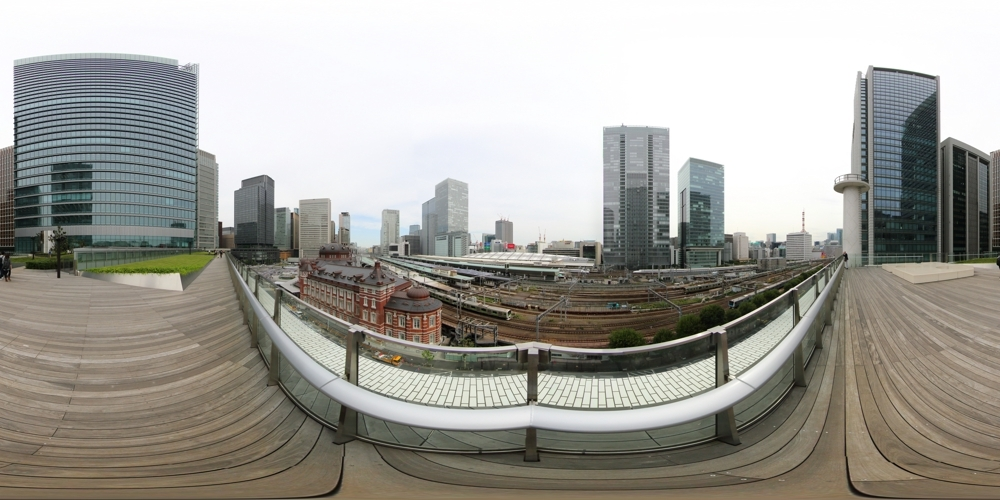
\includegraphics[scale=0.4]{figures/kadai2.jpg}
      \caption{全方位画像}
      \label{one}
    \end{center}
  \end{figure}
  \item 出力画像の画角 \\ $\Theta$(横方向) = 45°、$\Phi$(縦方向) = 45°
  \item 視線ベクトル \\ $\theta$(横方向) = -45°、$\phi$(縦方向) = -20°、$\psi$(光軸方向) = 45°
\end{itemize}

\subsubsection{出力}
\hyperref[one]{図\ref{one}}の全方位画像から、\hyperref[two]{図\ref{two}}の透視投影画像が出力された。 \\
 画素が荒くなってしまったが、視線ベクトルを指定することで狙った方角の透視投影画像が出力できていることがわかる。
\begin{figure}[!ht]
  \begin{center}
    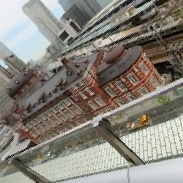
\includegraphics[scale=1.0]{figures/img_perspective.jpg}
    \caption{透視投影画像}
    \label{two}
  \end{center}
\end{figure}

\section{課題3.bashを用いた画像生成}
実装方法について、以下の節でまとめる。

\subsection{プログラムの引数の変更}
bashで扱いやすいようにプログラムの入力を変更する。ここでは、プログラムの引数として、水平方向の視線ベクトルを与える。
\subsection{シェルスクリプトの作成}
ソースコード\ref{fuga}は視線角度を$-\pi$から$\pi$まで10度ずつずらしpythonプログラムを実行するシェルスクリプトである。
\begin{lstlisting}[caption=連続な透視投影画像を表示,label=fuga]
  #!/bin/bash

  for i in $(seq 0 36)
  do
    python3 moveviewpoint.py kadai2.jpg input.csv $i
  done
\end{lstlisting}
また、シェルスクリプトの作成に合わせて、透視投影画像を表示するpythonプログラムも一部変更した。

\subsection{課題3の実行}
\subsubsection{入力}
入力画像、画角は課題2と同じ。高軸方向の視線ベクトルは$\psi = 0$とした。
\subsubsection{出力}
全37枚の画像が表示された。その中で一部の画像を下に示す。
\hyperref[three]{図\ref{three}}と\hyperref[four]{図\ref{four}}を見ると、右方向に平行移動していることがわかる。
また、\hyperref[three]{図\ref{three}}と\hyperref[six]{図\ref{six}}は同じになった。
これにより、透視投影画像の視点が水平方向に一周していることがわかる。

\begin{figure}[htbp]
  \begin{tabular}{cc}
    \begin{minipage}[t]{0.45\hsize}
      \centering
      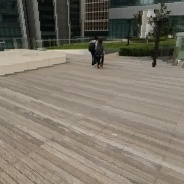
\includegraphics[keepaspectratio, scale=0.8]{figures/img_perspective0.jpg}
      \caption{$\theta$(横方向) = -180°}
      \label{three}
    \end{minipage} &
    \begin{minipage}[t]{0.45\hsize}
      \centering
      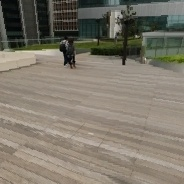
\includegraphics[keepaspectratio, scale=0.8]{figures/img_perspective1.jpg}
      \caption{$\theta$(横方向) = -170°}
      \label{four}
    \end{minipage} \\
 
    \begin{minipage}[t]{0.45\hsize}
      \centering
      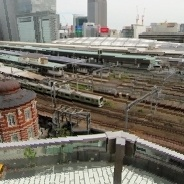
\includegraphics[keepaspectratio, scale=0.8]{figures/img_perspective18.jpg}
      \caption{$\theta$(横方向) = 0°}
      \label{five}
    \end{minipage} &
    \begin{minipage}[t]{0.45\hsize}
      \centering
      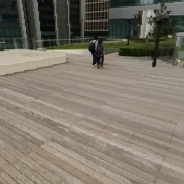
\includegraphics[keepaspectratio, scale=0.8]{figures/img_perspective36.jpg}
      \caption{$\theta$(横方向) = 180°}
      \label{six}
    \end{minipage} 
  \end{tabular}
\end{figure}

%参考文献
\begin{thebibliography}{99}
\bibitem{bib_1} 菅谷保之, 360 度画像からの透視投影画像の生成 (3), 4~5p, 最終更新日 2023年4月5日.
\end{thebibliography}

\end{document}
